% ------------------------------------------------------------------------------
% Resultados
% ------------------------------------------------------------------------------

\chapter{Resultados}

Neste capítulo, são apresentados e analisados os resultados obtidos a partir das simulações computacionais do modelo de queda livre. São exibidos os principais gráficos gerados, bem como tabelas que sintetizam os dados numéricos relevantes para a avaliação do comportamento do sistema e da acurácia dos métodos utilizados. A seguir, são discutidos os resultados à luz dos objetivos propostos.

Para facilitar a consulta, os principais resultados gráficos deste capítulo podem ser referenciados como: Figura~\ref{fig:particula_multidt} (partícula sem resistência), Figura~\ref{fig:linear_multidt} (corpo rígido com resistência linear), Figura~\ref{fig:quadratica_multidt} (corpo rígido com resistência quadrática) e Figura~\ref{fig:acuracia_graficos} (acurácia dos métodos numéricos). A tabela comparativa de acurácia está na Tabela~\ref{tab:tabela_acuracia}.




Os gráficos a seguir ilustram a evolução das principais variáveis do sistema ao longo do tempo, bem como a comparação entre diferentes cenários simulados.

\section{Resultados para o Modelo de uma Partícula em Queda Livre}
Foram realizados experimentos simulando a queda livre de uma partícula, variando o passo de tempo ($\Delta t$) para analisar o impacto na precisão dos resultados. Os gráficos a seguir apresentam, respectivamente, a posição, velocidade e aceleração em função do tempo para diferentes valores de $\Delta t$.
\begin{figure}[H]
	\centering
	\begin{subfigure}[b]{0.32\textwidth}
		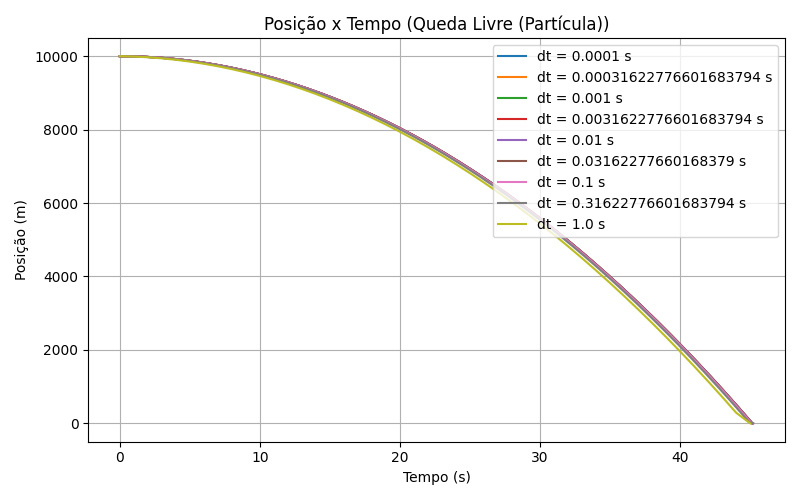
\includegraphics[width=\textwidth]{./figuras/graficos/queda_livre_particula/grafico_posicao_tempo_multidt}
		\caption{Posição}
	\end{subfigure}
	\hfill
	\begin{subfigure}[b]{0.32\textwidth}
		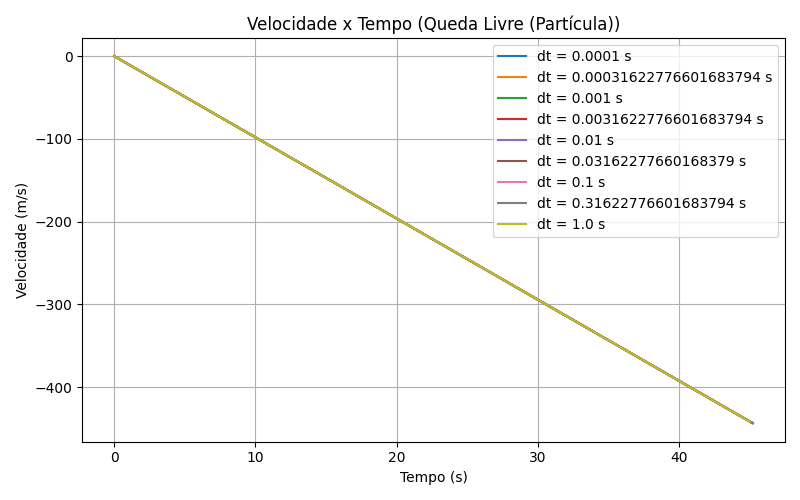
\includegraphics[width=\textwidth]{./figuras/graficos/queda_livre_particula/grafico_velocidade_tempo_multidt}
		\caption{Velocidade}
	\end{subfigure}
	\hfill
	\begin{subfigure}[b]{0.32\textwidth}
		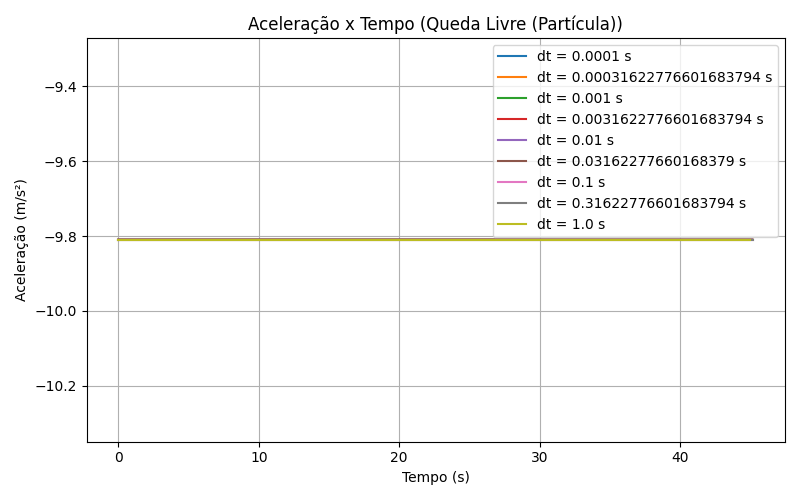
\includegraphics[width=\textwidth]{./figuras/graficos/queda_livre_particula/grafico_aceleracao_tempo_multidt}
		\caption{Aceleração}
	\end{subfigure}
	\caption{Resultados da simulação da queda livre de uma partícula para diferentes passos de tempo: (a) posição, (b) velocidade e (c) aceleração em função do tempo.}
	\label{fig:particula_multidt}
\end{figure}
\noindent
Para o modelo de queda livre sem resistência do ar, observa-se que a variação do passo de tempo ($\Delta t$) não altera significativamente as curvas de posição, velocidade e aceleração, desde que $\Delta t$ seja suficientemente pequeno. As trajetórias permanecem suaves e próximas da solução analítica, evidenciando a robustez do método numérico para esse caso. Apenas para valores grandes de $\Delta t$ surgem pequenas discrepâncias, principalmente na aceleração, reforçando a importância de uma escolha adequada do passo para garantir precisão.

\section{Resultados para o Modelo Corpo Rígido com Resistência Linear}
Para o corpo rígido com resistência linear (Lei de Stokes), os gráficos mostram a evolução das variáveis para diferentes passos de tempo.
\begin{figure}[H]
	\centering
	\begin{subfigure}[b]{0.32\textwidth}
		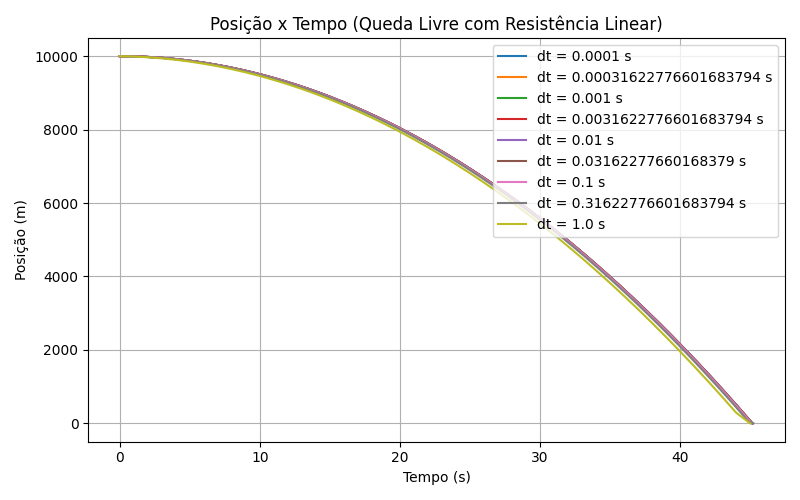
\includegraphics[width=\textwidth]{./figuras/graficos/queda_livre_corpo_rigido/linear/grafico_posicao_tempo_linear}
		\caption{Posição}
	\end{subfigure}
	\hfill
	\begin{subfigure}[b]{0.32\textwidth}
		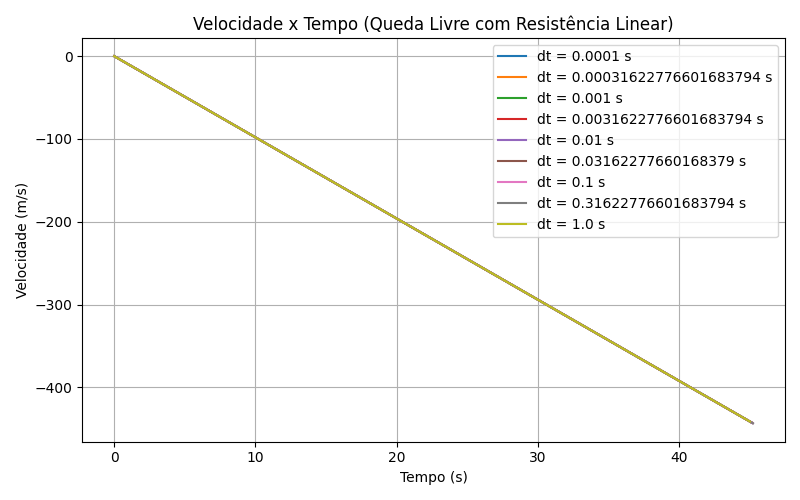
\includegraphics[width=\textwidth]{./figuras/graficos/queda_livre_corpo_rigido/linear/grafico_velocidade_tempo_linear}
		\caption{Velocidade}
	\end{subfigure}
	\hfill
	\begin{subfigure}[b]{0.32\textwidth}
		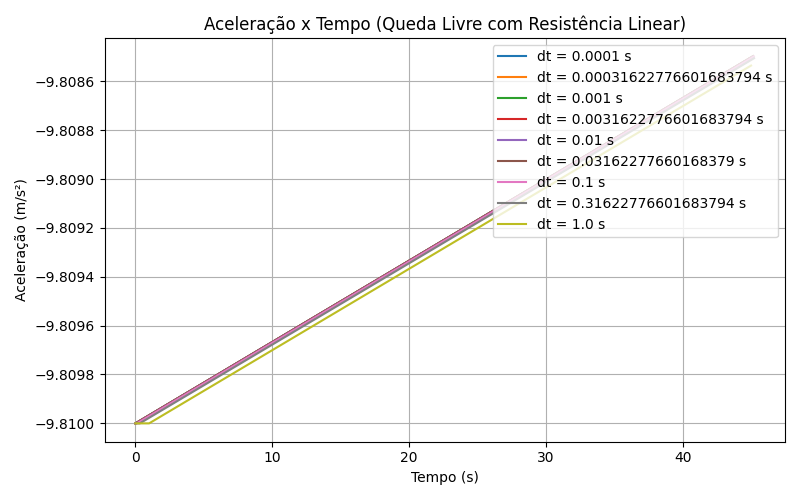
\includegraphics[width=\textwidth]{./figuras/graficos/queda_livre_corpo_rigido/linear/grafico_aceleracao_tempo_linear}
		\caption{Aceleração}
	\end{subfigure}
	\caption{Resultados da simulação do corpo rígido com resistência linear: (a) posição, (b) velocidade e (c) aceleração em função do tempo.}
	\label{fig:linear_multidt}
\end{figure}
\noindent
No caso do corpo rígido com resistência linear, os gráficos mostram que a posição e a velocidade convergem para valores de equilíbrio ao longo do tempo, caracterizando a velocidade terminal. Para passos de tempo pequenos, as curvas numéricas acompanham bem a solução teórica, mas, à medida que $\Delta t$ aumenta, surgem desvios mais perceptíveis, especialmente na velocidade e aceleração, que apresentam oscilações e perda de suavidade. Isso evidencia que, nesse modelo, a escolha de um $\Delta t$ adequado é ainda mais relevante para garantir resultados confiáveis.

\section{Resultados para o Modelo Corpo Rígido com Resistência Quadrática}
Para o corpo rígido com resistência quadrática, os gráficos a seguir apresentam a posição, velocidade e aceleração em função do tempo para diferentes passos de tempo.
\begin{figure}[H]
	\centering
	\begin{subfigure}[b]{0.32\textwidth}
		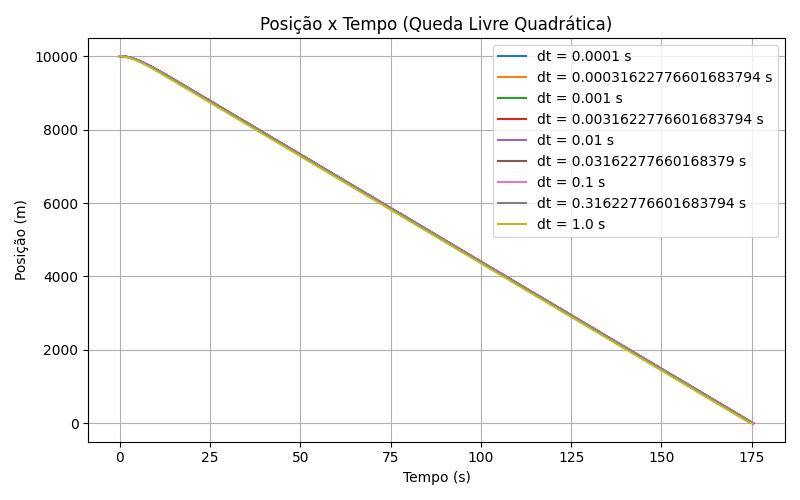
\includegraphics[width=\textwidth]{./figuras/graficos/queda_livre_corpo_rigido/quadratica/grafico_posicao_tempo_quadratica_multidt}
		\caption{Posição}
	\end{subfigure}
	\hfill
	\begin{subfigure}[b]{0.32\textwidth}
		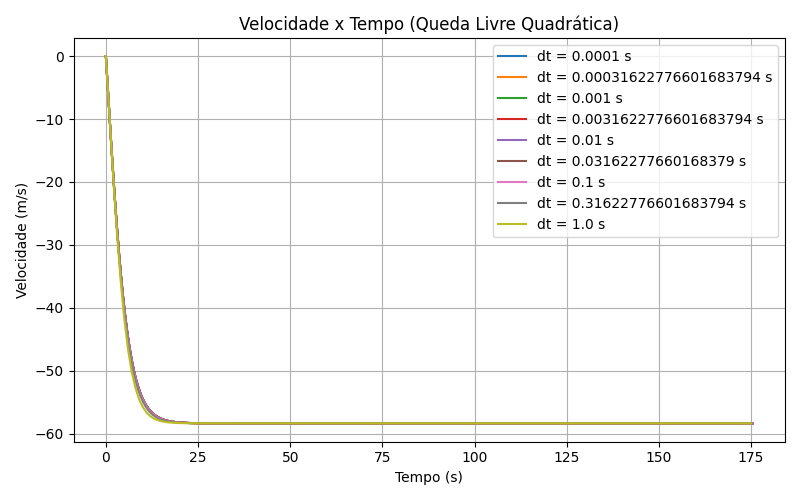
\includegraphics[width=\textwidth]{./figuras/graficos/queda_livre_corpo_rigido/quadratica/grafico_velocidade_tempo_quadratica_multidt}
		\caption{Velocidade}
	\end{subfigure}
	\hfill
	\begin{subfigure}[b]{0.32\textwidth}
		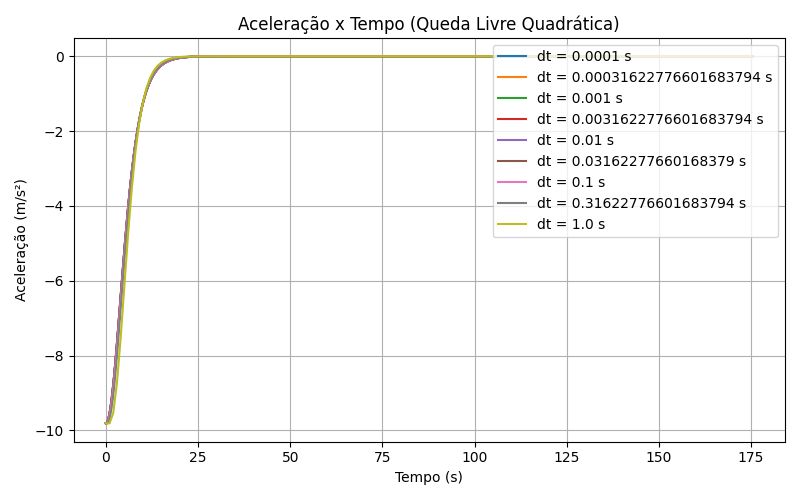
\includegraphics[width=\textwidth]{./figuras/graficos/queda_livre_corpo_rigido/quadratica/grafico_aceleracao_tempo_quadratica_multidt}
		\caption{Aceleração}
	\end{subfigure}
	\caption{Resultados da simulação do corpo rígido com resistência quadrática: (a) posição, (b) velocidade e (c) aceleração em função do tempo.}
	\label{fig:quadratica_multidt}
\end{figure}
\noindent
Para o modelo corpo rígido com resistência quadrática, observa-se que a influência do passo de tempo ($\Delta t$) é ainda mais acentuada. Com $\Delta t$ pequeno, as curvas de posição, velocidade e aceleração seguem de perto a solução analítica, mostrando a desaceleração rápida até atingir a velocidade terminal mais baixa entre os modelos. No entanto, para valores maiores de $\Delta t$, os resultados numéricos apresentam maiores oscilações e desvios, principalmente na aceleração, tornando evidente a necessidade de discretização fina para garantir precisão neste regime.

\section{Resultados da Acurácia}
Por fim, a acurácia dos métodos numéricos foi avaliada para cada modelo, variando o passo de tempo. Os gráficos a seguir mostram o erro relativo em função de $\Delta t$ para cada caso e a comparação geral.
\begin{figure}[H]
    \centering
    \begin{subfigure}[b]{0.32\textwidth}
        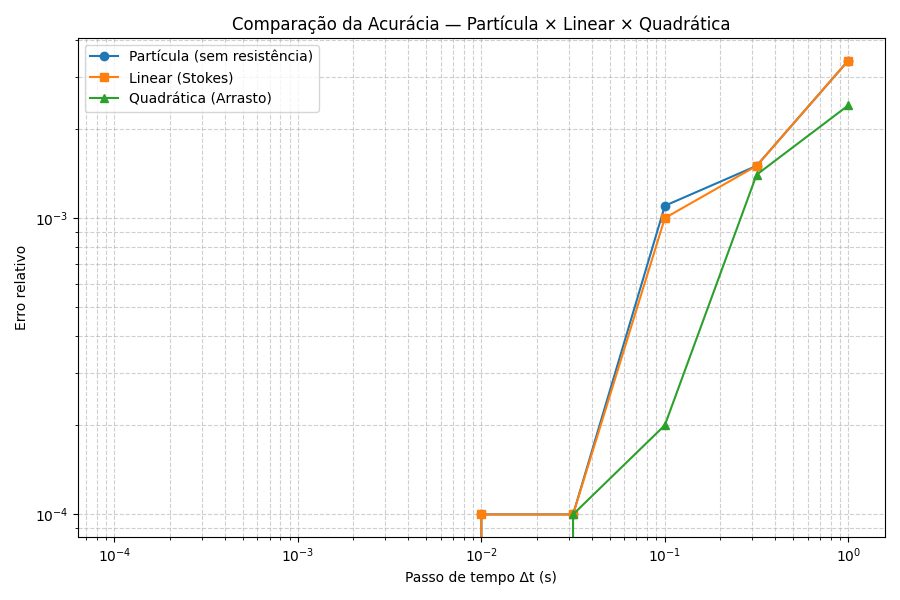
\includegraphics[width=\textwidth]{./figuras/graficos/acuracia/log/acuracia_comparativa_log.png}
        \caption{Partícula sem resistência do ar}
    \end{subfigure}
    \hfill
    \begin{subfigure}[b]{0.32\textwidth}
        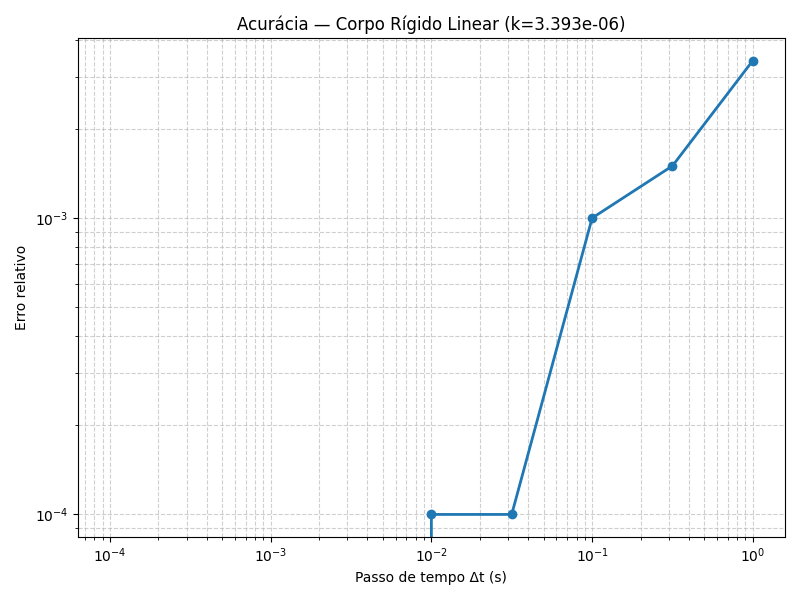
\includegraphics[width=\textwidth]{./figuras/graficos/acuracia/log/acuracia_linear_log.png}
        \caption{Corpo rígido com resistência linear}
    \end{subfigure}
    \hfill
    \begin{subfigure}[b]{0.32\textwidth}
        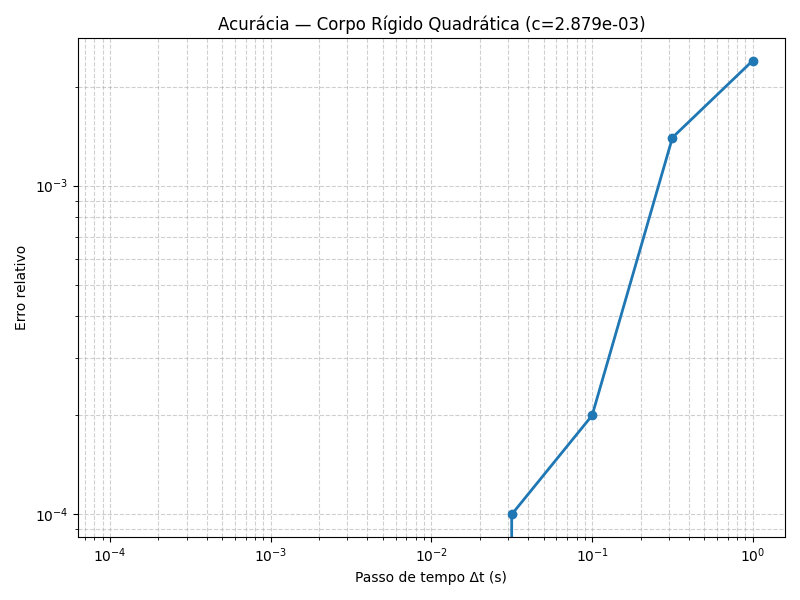
\includegraphics[width=\textwidth]{./figuras/graficos/acuracia/log/acuracia_quadratica_log.png}
        \caption{Corpo rígido com resistência quadrática}
    \end{subfigure}
    \caption{Acurácia do método numérico para (a) partícula sem resistência do ar, (b) corpo rígido com resistência linear e (c) corpo rígido com resistência quadrática.}
    \label{fig:acuracia_graficos}
\end{figure}

Os resultados de acurácia mostram que, para todos os modelos, o erro relativo médio permanece muito baixo quando se utiliza um passo de tempo pequeno, garantindo alta precisão numérica. No entanto, à medida que $\Delta t$ aumenta, os modelos com resistência do ar — especialmente o quadrático — apresentam crescimento mais acentuado do erro, principalmente na velocidade e aceleração. Isso reforça a necessidade de uma escolha criteriosa do passo de tempo para evitar perdas de precisão, sendo a posição a variável menos sensível e a aceleração a mais afetada pelos efeitos numéricos.

De modo geral, os experimentos numéricos evidenciam que a escolha do passo de tempo ($\Delta t$) é fundamental para garantir precisão, especialmente nos modelos com resistência do ar. Enquanto o modelo sem resistência é pouco sensível a $\Delta t$, os modelos linear e, principalmente, quadrático exigem discretizações mais refinadas para evitar oscilações e erros acentuados, sobretudo na aceleração. Assim, a análise computacional reforça a importância de parâmetros adequados para a confiabilidade dos resultados em diferentes regimes de queda livre.



